\chapter{Concepts in Spin Conductance Models}

\section{Converting from $\Pi$-model to T-model}

Depending on the situation, it might be easier to work with the $\Pi$-model or the T-model. However, the derivation of the conductance matrix is straightforward using the $\Pi$-model, as described earlier. Hence, we need to derive the equivalent conductances in the T-model from the $\Pi$-model conductances. Before we begin, note that in the spin conductance model, the conductances are tensors instead of scalars. Hence, it is important to preserve the order of multiplication.

Let us begin by looking at the $\Pi$-model as shown in Fig.~\ref{fig:modelDiagrams}. We can first write the following equations:
\begin{IEEEeqnarray}{rCl}
I_{out}&=&I_{p}+I_{2} \label{eq:piIout}\\
I_{in}&=&I_{p}-I_{1} \label{eq:piIin}\\
I_{1}&=&G_{sf\pi}V_{1} \label{eq:piI1}\\
I_{2}&=&G_{sf\pi}V_{2} \label{eq:piI2} \\
I_{p}&=&G_{se\pi}(V_{2}-V_{1}) \label{eq:piIp}
\end{IEEEeqnarray}Then, we add Eqs.~(\ref{eq:piIout}) and (\ref{eq:piIin}) to get \begin{IEEEeqnarray}{rCl}
I_{out}+I_{in}&=&2I_{p}+I_{2}-I_{1} \label{eq:piCurrSum}
\end{IEEEeqnarray}Substituting Eqs.~(\ref{eq:piI1}), (\ref{eq:piI2}) and (\ref{eq:piIp}) into Eq.~(\ref{eq:piCurrSum}), we obtain \begin{IEEEeqnarray}{rCl}
I_{out}+I_{in}&=&2G_{se\pi}(V_{2}-V_{1})+G_{sf\pi}V_{2}-G_{sf\pi}V_{1} \nonumber \\
&=& 2G_{se\pi}(V_{2}-V_{1})+G_{sf\pi}(V_{2}-V_{1}) \label{eq:piCurrSum2} \\
&=& (2G_{se\pi}+G_{sf\pi})(V_{2}-V_{1}) \nonumber
\end{IEEEeqnarray}Next, we subtract Eq.~(\ref{eq:piIin}) from Eq.~(\ref{eq:piIout}) to get \begin{IEEEeqnarray}{rCl}
I_{out}-I_{in}&=&I_{2}+I_{1} \label{eq:piCurrDiff}
\end{IEEEeqnarray}Substituting Eqs.~(\ref{eq:piI1}) and (\ref{eq:piI2}) into Eq.~\ref{eq:piCurrDiff}, we get \begin{IEEEeqnarray}{rCl}
I_{out}-I_{in}&=&G_{sf\pi}(V_{2}+V_{1}) \label{eq:piCurrDiff2}
\end{IEEEeqnarray}

Now, let us look at the T-model in Fig.~\ref{fig:modelDiagrams}. The objective is to write $I_{out}+I_{in}$ and $I_{out}-I_{in}$, and compare them to the equations for the $\Pi$-model so that we can obtain equations for $G_{seT}$ and $G_{sfT}$ in terms of $G_{se\pi}$ and $G_{sf\pi}$. First, we can write the following equations for the T-model:\begin{IEEEeqnarray}{rCl}
I_{out}&=&G_{seT}(V_{2}-V_{m}) \label{eq:tIout}\\
I_{in}&=&G_{seT}(V_{m}-V_{1}) \label{eq:tIin}\\
I_{m}&=&G_{sfT}V_{m} \label{eq:tIm}\\
I_{out}&=&I_{in}+I_{m} \label{eq:tKCL1}
\end{IEEEeqnarray}Adding Eqs.~(\ref{eq:tIout}) and (\ref{eq:tIin}), we get \begin{IEEEeqnarray}{rCl}
I_{out}+I_{in}&=&G_{seT}(V_{2}-V_{1}) \label{eq:tCurrSum}
\end{IEEEeqnarray}\begin{figure}
\centering
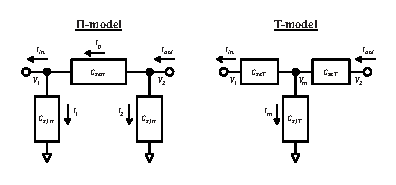
\includegraphics[scale=1.75]{ResearchNotes_SpinConductanceModels/figs/2Ports}
\caption{These circuit diagrams show how conductances are arranged in the $\Pi$-model and the T-model.}
\label{fig:modelDiagrams}
\end{figure}Subtracting Eq.~(\ref{eq:tIin}) from Eq.~(\ref{eq:tIout}), we get \begin{IEEEeqnarray}{rCl}
I_{out}-I_{in}&=&G_{seT}(V_{2}+V_{1}-2V_{m}) \label{eq:tCurrDiff}
\end{IEEEeqnarray}Then, we rearrange Eq.~(\ref{eq:tKCL1}) and substituting into Eq.~(\ref{eq:tIm}):\begin{IEEEeqnarray}{rCl}
I_{out}-I_{in}&=&G_{sfT}V_{m} \label{eq:tCurrDiff2}
\end{IEEEeqnarray}Pre-multiplying both sides of Eq.~(\ref{eq:tCurrDiff2}) with $G^{-1}_{sfT}$:\begin{IEEEeqnarray}{rCl}
V_{m}&=&G^{-1}_{sfT}(I_{out}-I_{in}) \label{eq:tVm}
\end{IEEEeqnarray}Substituting Eq.~(\ref{eq:tVm}) into Eq.~(\ref{eq:tCurrDiff}):\begin{IEEEeqnarray}{rCl}
I_{out}-I_{in}&=&G_{seT}(V_{2}+V_{1})-2G_{seT}G^{-1}_{sfT}(I_{out}-I_{in}) \label{eq:tCurrDiff3}
\end{IEEEeqnarray}Rearranging Eq.~(\ref{eq:tCurrDiff3}):\begin{IEEEeqnarray}{rCl}
G_{seT}(V_{2}+V_{1})&=&(I+2G_{seT}G^{-1}_{sfT})(I_{out}-I_{in}) \label{eq:tCurrDiff4}
\end{IEEEeqnarray}where $I$ is the identity matrix.

Comparing Eqs.~(\ref{eq:piCurrSum2}) and (\ref{eq:tCurrSum}), we get \begin{IEEEeqnarray}{rCl}
G_{seT}&=&2G_{se\pi}+G_{sf\pi} \label{eq:gset}
\end{IEEEeqnarray}Next, we compare Eqs.~(\ref{eq:piCurrDiff2}) and (\ref{eq:tCurrDiff4}) and obtain \begin{IEEEeqnarray}{rCl}
(I+2G_{seT}G^{-1}_{sfT})G_{sf\pi}&=&G_{seT} \label{eq:gset2}
\end{IEEEeqnarray}Substituting Eq.~(\ref{eq:gset}) into the right-hand side of (\ref{eq:gset2}): \begin{IEEEeqnarray}{rCl}
(I+2G_{seT}G^{-1}_{sfT})G_{sf\pi}&=&2G_{se\pi}+G_{sf\pi} \\
G_{sf\pi}+2G_{seT}G^{-1}_{sfT}G_{sf\pi}&=&2G_{se\pi}+G_{sf\pi} \\
2G_{seT}G^{-1}_{sfT}G_{sf\pi}&=&2G_{se\pi} \label{eq:gsePiA}
\end{IEEEeqnarray}Post-multiplying both sides of Eq.~(\ref{eq:gsePiA}) by $\frac{G^{-1}_{sf\pi}}{2}$, we obtain \begin{IEEEeqnarray}{rCl}
G_{seT}G^{-1}_{sfT}&=&G_{se\pi}G^{-1}_{sf\pi} \label{eq:gProd}
\end{IEEEeqnarray}Post-multiplying both sides of Eq.~(\ref{eq:gProd}) by $G_{sfT}$:\begin{IEEEeqnarray}{rCl}
G_{seT}&=&G_{se\pi}G^{-1}_{sf\pi}G_{sfT} \label{eq:gset3}
\end{IEEEeqnarray}Substitute Eq.~(\ref{eq:gset}) into Eq.~(\ref{eq:gset3}), we get:\begin{IEEEeqnarray}{rCl}
G_{se\pi}G^{-1}_{sf\pi}G_{sfT}&=&2G_{se\pi}+G_{sf\pi} \label{eq:gsft}
\end{IEEEeqnarray}Pre-multiplying both sides of Eq.~(\ref{eq:gsft}) by $G^{-1}_{se\pi}$: \begin{IEEEeqnarray}{rCl}
G^{-1}_{sf\pi}G_{sfT}&=&2I+G^{-1}_{se\pi}G_{sf\pi} \label{eq:gsft2}
\end{IEEEeqnarray}Finally, pre-multiply both sides of Eq.~(\ref{eq:gsft2}) by $G_{sf\pi}$: \begin{IEEEeqnarray}{rCl}
G_{sfT}&=&G_{sf\pi}G^{-1}_{se\pi}G_{sf\pi}+2G_{sf\pi} \label{eq:gsft3}
\end{IEEEeqnarray}

Thus, we can convert from the $\Pi$-model to the T-model using \begin{IEEEeqnarray}{rCl}
G_{seT}&=&2G_{se\pi}+G_{sf\pi} \\
G_{sfT}&=&G_{sf\pi}G^{-1}_{se\pi}G_{sf\pi}+2G_{sf\pi}
\end{IEEEeqnarray}
